\chapter{Simulatieresultaten}
\label{resultaten}

\section{Wijzigingen aan de implementatie}
\label{wijzigingen}
\subsection{Het kickstartprobleem}
\npar In principe zou bovenstaande uitwerking moeten werken.  Helaas, dit was buiten ns-click gerekend waarin blijkbaar enkele rare implementatiekeuzes gemaakt werden of waar gewoon nog een aantal bugs in zitten.  Zo hadden we de rare situatie dat wanneer de dispatcher ge�mplementeerd was zoals het hoort en het downstreamverkeer dus geblokkeerd werd totdat een upstreampakket ontvangen werd, het geheel niet werkte.  Pas vanaf 3.1~s kon het eerste upstreampakket verzonden worden.  Wanneer we de dispatcher initialiseren, en deze vanaf het begin downstreamverkeer doorlaat naar een vooraf gekozen RAU, werkt alles naar behoren.  Althans zo lang de trein zich ter hoogte van de eerste RAU bevindt.  Vanaf er overgeschakeld wordt op de tweede RAU, geraakt er slechts 10\% van het upstreamverkeer meer verzonden, terwijl er voor het downstreamverkeer geen probleem is.  We hebben geen idee hoe dit komt, maar de kans bestaat dat de oorzaak in dezelfde richting moet gezocht worden als deze die problemen heeft bij de eerste RAU wanneer de dispatcher oorspronkelijk al het verkeer blokkeert.  Dit probleem werd reeds aangebracht als het \textit{kickstartprobleem} in sectie \ref{nsclick}.

\subsection{Verwisselen AP- en station-functionaliteit}
\npar Zoals uit bovenstaande paragraaf blijkt, moet het eerste verkeer afkomstig zijn van het AP.  Echter, als we aan het principe willen vasthouden dat het eerste verkeer afkomstig moet zijn van de trein, dan lijkt de conclusie eenvoudig: plaats het AP op de trein en laat de centrale voor draadloze client doorgaan.  In wezen mag dit geen verschil maken aangezien we toch met ��n station per AP werken.  Station en AP vormen samen niet meer dan een tunnel waardoor gewoon ethernet- of IP-verkeer gestuurd kan worden.  Het enige verschil is dat het AP normaal beacon frames verstuurt en dat het station zich moet authenticeren en associ�ren met het AP.  Bovendien levert dit een bijkomend voordeel op.  Om een goede werking mogelijk te maken, moet de trein regelmatig verkeer naar de centrale sturen.  Indien er geen verkeer voorhanden is, gingen we random informatie versturen.  Als de trein echter beacon frames uitzendt, dan hebben we meteen een periodieke bron van verkeer en moet daar ook niets meer voor voorzien worden.

\npar Na het verwisselen van de AP- en station-functionaliteiten blijkt alles naar behoren te werken.  Het verkeer start, met de correcte dispatcher, onmiddellijk ipv na 3.1~s en er zijn geen problemen meer nadat op een nieuw RAU werd overgegaan.  De bespreking van de resultaten is dan ook van toepassing op deze kleine ingreep, die hoegenaamd niets verandert aan de werking van het geheel buiten deze simulatie-omgeving.

\section{Referentie}
\npar Vooraleer over te gaan tot een gedetailleerde bespreking van de resultaten, is het best eerst over referentiewaarden te beschikken van een klassiek systeem.  Het is onzinnig om een vrijwillige handover als basis voor onze vergelijking te nemen.  Dit is immers afhankelijk van de implementatie van het mechanisme dat bepaalt wanneer het signaal van het oude AP te zwak wordt en dat van het nieuwe sterk genoeg geworden is, en er tot een handover overgegaan wordt.  Bovendien wacht een standaard client nog op een ACK-bericht na het sturen van de disassociate, wat bij een slecht signaal wel heel lang kan duren na enkele retries.  In onze simulaties beslissen we zelf wanneer we overschakelen en is het signaal tijdens het overschakelen altijd goed genoeg.  Van zodra we de handover uitgevoerd hebben, wordt het signaal enkel nog beter.  We vergelijken dus best met een test met gedwongen handovers, waarbij we zelf beslissen om het station te laten associ�ren met een nieuw AP terwijl de signaalkwaliteit van beide AP's constant blijft op een goede waarde.  Testresultaten met gedwongen handovers op het goede moment leveren betere resultaten op dan wanneer de beslissing overgelaten wordt aan het station dat geen idee heeft waar het zich bevindt en welk signaal er sterker of zwakker zal worden.  Als ons systeem even goed of beter scoort dan een vergelijkbaar systeem met gedwongen handovers, dan weten we ook waar we staan ten opzichte van de situatie met door het station ge�nitieerde handovers.

\subsection{Hardwaretest}
\npar Een eerste test waarmee we kunnen vergelijken, is een hardwaretest die deze zomer uitgevoerd werd tijdens een stage.  Hiervoor hernemen we grafieken C.8 en C.9 van pagina's 43 en 44 van het stageverslag \cite{stage} over als figuren \ref{Chantry1} en \ref{Chantry2}.  Beiden zijn het resultaat van het sturen van een UDP-teststroom van +/-~1~Mbps vanaf een server in het bovenliggend netwerk naar het station.  Figuur \ref{Chantry2} is een detailopname van de handover.  5~s na het begin van de datastroom werd tot een handover overgegaan, die duidelijk te herkennen is aan de \textit{gap} van +/-~300~ms in de grafiek gedurende dewelke geen verkeer door de draadloze brug mogelijk was.  De AP's zijn Chantry Beaconpoints, die sinds de overname door Siemens door het leven gaan als Siemens HiPath.  Het station is een door Linux aangedreven laptop met Intel IPW2200 interne WiFi-kaart.

\begin{figure}[ht]
  \begin{center}
    \includegraphics[width=.5\textwidth]{Chantry1.png}
    \caption{Analyse van een UDP-teststroom aan +/-~1~Mbps met na de $26^e$ seconde (5~s na het begin van de datastroom) een handover.  De horizontale as is de tijdsas, verticaal staat de doorstroom in \textit{Bytes per tick}.  E�n tick is 0,1~s waardoor de waarde 10.000 op de grafiek overeenkomt met 100.000~Bps of 800~Kbps.\label{Chantry1}}
  \end{center}
\end{figure}

\begin{figure}[ht]
  \begin{center}
    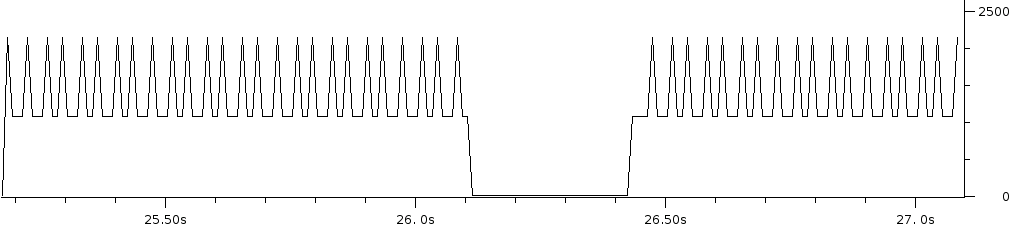
\includegraphics[width=\textwidth]{Chantry2.png}
    \caption{Detail van de handover van figuur \ref{Chantry1}: tijdens een UDP-teststroom aan +/-~1~Mbps werd na de $26^e$ seconde (5~s na het begin van de stroom) tot een handover overgegaan.  De horizontale as is de tijdsas, verticaal staat de doorstroom in \textit{Bytes per tick}.  E�n tick is 0,01~s waardoor de waarde 1.000 op de grafiek overeenkomt met 100.000~Bps of 800~Kbps.\label{Chantry2}}
  \end{center}
\end{figure}

\npar Bij deze vergelijkingsbasis dienen uiteraard de nodige kritische bedenkingen aangebracht te worden.  Deze hardwaresimulatie werd uitgevoerd op een platform dat ontwikkeld werd voor snelle handovers.  Bovendien werd hier gewerkt met de IEEE~802.11g standaard in plaats van de b-standaard die wij gebruiken.  Verder is ns-click echt niet geschikt voor doorstroomtesten aangezien er een beperking zit op de verkeersstroom die men met ns door een draadloze brug kan sturen.

\subsection{Simulatie met conventionele AP's in ns-click}
\label{resultaten-simulatie-ap}
\npar Een betere basis om mee te vergelijken, zou het nabootsen van een klassieke situatie zijn in ns-click.  Op die manier worden simulatieresultaten afkomstig van dezelfde simulator, met dezelfde eigenschappen en beperkingen, met elkaar vergeleken.  Dit is echter ook niet evident.  De modellen voor een AP en station die gebruikt worden in ns-click zijn slechts basismodellen.  De standaard wordt (grotendeels) gevolgd, maar het blijft toch mogelijk om pakketten te versturen over de draadloze brug ook zonder dat het station geassocieerd is met het AP.  Een voorbeeld van een dergelijke gecapteerde pakketstroom is te vinden in \ref{details-pakketstroom}.  Als het station overschakelt op een nieuw AP, dan kan deze al onmiddellijk upstreampakketten sturen via het nieuwe AP, nog voor het geassocieerd is, waarna de bovenliggende switch onmiddellijk de downstreampakketten naar het nieuwe AP stuurt.  De pakketten in de buffers van het oude AP gaan dan verloren, tenzij deze door de node in het bovenliggend netwerk opnieuw verstuurd worden.  Indien het station geen verkeer naar een node in het bovenliggende netwerk stuurt, zal de switch ook nooit weten dat het station bereikt moet worden via een nieuw AP en zullen de pakketten nog steeds enkel bij het oude AP toekomen alwaar ze de buffers laten overlopen en verloren gaan. In bovenstaande hardwaretest gaan geen pakketten verloren: het oude AP stuurt deze naar het nieuwe AP via het Inter Access Point Protocol (IAPP), dat momenteel gestandaardiseerd wordt, of via een eigen IAPP.  Het is echter niet omdat men direct pakketten kan versturen na het overschakelen op een nieuw AP, dat er geen handovertijd zou zijn.  Het omschakelen op een nieuwe frequentie en het synchroniseren met een zender op die frequentie vergt ook enige tijd.

\begin{figure}[ht]
  \begin{center}
    \includegraphics[width=.75\textwidth]{2ap}
    \caption{Testopstelling voor het bepalen van een vergelijkingsbasis.\label{2ap}}
  \end{center}
\end{figure}

\npar Er werd een testopstelling aangemaakt in ns-click zoals afgebeeld in figuur \ref{2ap}.  De nodes zijn vast gepositioneerd op de opgegeven co�rdinaten.  Na 1~s stelt het station zich in op kanaal~1 en authenticeert het zich bij AP0 om 10~ms later ermee te associ�ren.  2~s na het begin van de simulatie wordt een UDP-teststroom aan een bitrate van 3,6 Mbps gestuurd van de server naar het station.  100~ms later begint een gelijkaardige bitstroom in de omgekeerde richting.  Na 2~s verandert het station naar kanaal~6 om zich te authenticeren bij AP1.  Dat er ondertussen al pakketten gestuurd worden, is af te lezen in bijlage \ref{details}: gedetailleerde resultaten.  De simulatie wordt afgebroken na 6~seconden.  De resultaten zijn grafisch uitgezet in figuur \ref{referentie}.  De zwarte lijn stelt de totale doorstroom door de draadloze link voor.  Groen en rood staan voor de stroom van het station naar de server, respectievelijk van de server naar het station.  Er is duidelijk een gap te zien op het moment dat overgeschakeld wordt op de nieuwe frequentie.  Dit moment is uitvergroot in figuur \ref{referentie-detail}.  Deze gap is 100~ms breed voor de rode lijn en 90~ms voor de andere lijnen.  Dit verschil is te verklaren door het feit dat pas vanaf het eerste upstream UDP-pakket de switch bereikt heeft, deze overschakelt en aankomende downlink UDP-pakketten naar het nieuwe AP stuurt.

\begin{figure}[ht]
  \begin{center}
    \includegraphics[width=.75\textwidth]{referentie}
    \caption{Doorstroom van een UDP-teststroom bij 2 gewone AP's.  De horizontale as is de tijdsas, verticaal staat de doorstroom in \textit{Bytes per tick}.  E�n tick is 0,1~s waardoor de waarde 100.000 op de grafiek overeenkomt met 1.000.000~Bps of 8~Mbps.\label{referentie}}
  \end{center}
\end{figure}


\begin{figure}[ht]
  \begin{center}
    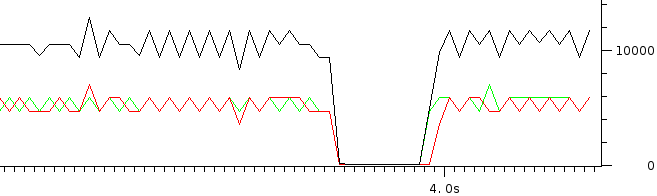
\includegraphics[width=.75\textwidth]{referentie-detail}
    \caption{Detailopname van de handover tijdens de doorstroom van een UDP-teststroom bij 2 gewone AP's, zoals weergegeven in figuur \ref{referentie}.  De horizontale as is de tijdsas, verticaal staat de doorstroom in \textit{Bytes per tick}.  E�n tick (hier ��n klein streepje op de horizontale as) is 0,01~s waardoor de waarde 10.000 op de grafiek overeenkomt met 1.000.000~Bps of 8~Mbps.\label{referentie-detail}}
  \end{center}
\end{figure}

\section{Resultaten van het systeem op basis van Radio-over-Fiber}
\npar Zoals vermeld in \ref{werking-systeem}, is dit een uiterst flexibel systeem.  Meerdere (kruisende) treinen, meerdere kanalen per trein, er is heel wat mogelijk.  We zullen in deze sectie een paar van deze voorbeelden uitwerken en de simulatieresultaten bespreken.  We beginnen uiteraard bij een basisgeval om de werking van het moving cell principe te illustreren.

\subsection{1 trein, 2 remote antenna units}
\label{1t2bs}
\npar De testopstelling is ge�llustreerd in figuur \ref{1trein2bs}.  Het bereik van de draadloze nodes is afgesteld op 105~m, zodat we een overlapzone van 10~m bekomen.  Het grote voordeel aan deze manier van werken, is dat wanneer er overgeschakeld wordt op een nieuwe RAU, eventuele data die nog onderweg is van de centrale naar de oude RAU alsnog afgeleverd kan worden op de trein.  De trein is ondertussen overgeschakeld op de nieuwe RAU en de signaalkwaliteit zal alleen maar verbeteren, tot wanneer de trein de RAU voorbijrijdt.

\begin{figure}[ht]
  \begin{center}
    \includegraphics[width=.75\textwidth]{1trein2bs}
    \caption{Testopstelling met 1 trein en 2 RAU's.\label{1trein2bs}}
  \end{center}
\end{figure}

\npar Initieel staat de trein stil op de beginpositie.  Het AP in de trein is reeds actief vanaf het begin en zendt op regelmatige tijdstippen beacon frames uit.  Na 1~s gaat het station in de centrale een probe request uitsturen naar het AP dat zich op de trein bevindt, van waaruit een antwoord teruggestuurd wordt.  500~ms later authenticeert het station zich, om 100~ms later te associ�ren met het AP.  2~seconden na het begin van de simulatie, start de trein zijn beweging aan 40~m/s, wat overeenkomt met 144~km/u.  Op seconde 3 start vervolgens een bitstroom aan 3,6~Mbps van de server naar de trein.  Om een nog onbekende reden is de troughput van de trein naar de centrale bijzonder laag.  De omgekeerde richting, van de server naar de trein, is echter het interessantst van al.  Het is deze stroom die naar de juiste RAU gerouteerd moet worden om op de trein terecht te komen.  Aan de trein zelf verandert er niets: het is steeds hetzelfde station (in de centrale) dat geassocieerd blijft met het AP in de trein en deze laatste verandert ook niet van frequentie of andere parameters.  Enkel in de centrale gebeurt de omschakeling naar de nieuwe RAU.  Na 8~s is het experiment voorbij.

\npar Een analyse van de bitstroom levert bijzonder interessante informatie op.  Het resultaat is grafisch weergegeven in figuur \ref{resultaten-1t2bs}.  In tegenstelling tot de referentiemetingen is hier helemaal geen gap of dipje te merken in de doorstroom.  De stroom is continu.

\begin{figure}[ht]
  \begin{center}
    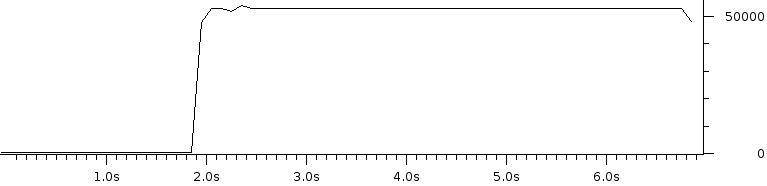
\includegraphics[width=.75\textwidth]{resultaten-1t2bs}
    \caption{Doorstroom van een UDP-teststroom bij het RoF-model.  De horizontale as is de tijdsas, verticaal staat de doorstroom in \textit{Bytes per tick}.  E�n tick is 0,1~s waardoor de waarde 50.000 op de grafiek overeenkomt met 500.000~Bps of 4~Mbps.\label{resultaten-1t2bs}}
  \end{center}
\end{figure}

\npar Een ander interessant experiment, is het meten van de bitstroom aan de centrale, meerbepaald het verkeer van en naar de RAU's.  Als we dat verkeer opsplitsen per RAU, zien we hoe lang de trein zich in de overlapzone bevindt en wanneer de centrale omgeschakeld is naar de nieuwe RAU.  Om een en ander beter zichtbaar te maken, sturen we ook een kleine UDP-teststroom van 76~kbps van de trein naar de server.  Op die manier hebben we iets meer verkeer en bekomen we kwalitatievere metingen.  De resultaten zijn te zien in figuur \ref{RoF-1t2rau-centrale}.  We zien dat vanaf het eerste pakket van de tweede RAU (paarse lijn) binnenkomt op seconde 4,35, de centrale overschakelt en het verkeer naar RAU0 (de rode lijn) volledig naar nul gaat.  Op de grafiek lijkt dit niet onmiddellijk te gaan, maar ongeveer 200~ms te duren.  Dit klopt niet: dit zou moeten een rechte verticale lijn zijn.  Dit is beter zichtbaar in een detailopname van de handover, weergegeven in figuur \ref{RoF-1t2rau-centrale-detail}.  De trein bevindt zich in de overlapzone als de uitgezonden pakketten opgepikt worden door zowel RAU0 en RAU1, wat op de grafiek te zien is als de zone waar de paarse en blauwe lijn samen verschillen van nul.  Dit is het geval vanaf 4,3~s tot 4,75~s.  De centrale is echter al vanaf het begin overgeschakeld, daar waar de groene lijn (het verkeer naar RAU1) de tijdsas verlaat.  Er is duidelijk te zien dat het verkeer, zowel van de server naar de trein als omgekeerd, niet onderbroken wordt.

\npar Figuur \ref{RoF-1t2rau-centrale-detail} lijkt grilliger, wat komt door de sterke uitvergroting van de tijdschaal.  Elke lage piek komt dan overeen met een binnenkomend of vertrekkend pakket, UDP-pakketten worden verzonden met een datainhoud van 1000 bytes.  Hier is de omschakeling van de centrale op RAU1 beter te zien: de rode en groene lijn zijn steiler en het gebied waar beiden van de tijdsas afwijken, is in verhouding tot de overlapzone (waar de blauwe en paarse lijn van de tijdsas afwijken) veel kleiner dan op figuur \ref{RoF-1t2rau-centrale}, wat duidelijk aangeeft dat de breedte van de groen-rode overlap een zuiver grafische oorzaak heeft.

\begin{figure}[ht]
  \begin{center}
    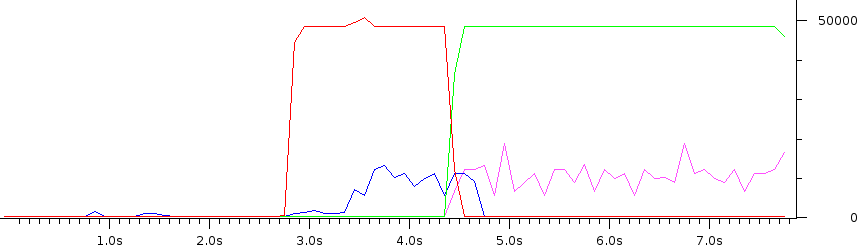
\includegraphics[width=.9\textwidth]{RoF-1t2rau-centrale.png}
    \caption{Pakketstromen tussen de centrale en de RAU's in het RoF-model.  De horizontale as is de tijdsas, verticaal staat de doorstroom in \textit{Bytes per tick}.  E�n tick is 0,1~s waardoor de waarde 50.000 op de grafiek overeenkomt met 500.000~Bps of 4~Mbps.  De rode en groene lijnen geven het verkeer van de centrale naar RAU0, respectievelijk RAU1, weer, terwijl de blauwe en paarse lijnen de stroom van RAU0 respectievelijk RAU1 naa de centrale voorstellen.\label{RoF-1t2rau-centrale}}
  \end{center}
\end{figure}


\begin{figure}[ht]
  \begin{center}
    \includegraphics[width=.9\textwidth]{RoF-1t2rau-centrale-detail.png}
    \caption{Detailopname van de pakketstromen tussen de centrale en de RAU's in het RoF-model.  De horizontale as is de tijdsas, verticaal staat de doorstroom in \textit{Bytes per tick}.  E�n tick is 0,01~s waardoor de waarde 5.000 op de grafiek overeenkomt met 500.000~Bps of 4~Mbps.  De rode en groene lijnen geven het verkeer van de centrale naar RAU0, respectievelijk RAU1, weer, terwijl de blauwe en paarse lijnen de stroom van RAU0 respectievelijk RAU1 naar de centrale voorstellen.\label{RoF-1t2rau-centrale-detail}}
  \end{center}
\end{figure}


\subsection{2 treinen, 3 remote antenna units}
\label{2t3bs}

\npar Zoals reeds meermaals in dit werk vermeld, is ons model bijzonder flexibel.  Er kunnen meerdere kruisende treinen zijn, of treinen die behoefte hebben aan een hogere bandbreedte, kunnen een bijkomend kanaal toegewezen krijgen.  Uiteraard is het aangewezen ook dit even experimenteel na te gaan.  Hiervoor cre�ren we een opstelling zoals weergegeven in figuur \ref{2trein3bs}.  Wanneer we naar beide treinen afzonderlijk maar simultaan een teststroom willen sturen van 3,2~Mbps, komen we al snel een beperkende factor tegen.  Na +/-~7~seconden, als de eerste trein zich in het overlapgebied van RAU0 en RAU1 bevindt en de tweede in dat van RAU1 en RAU2, loopt de eerste wachtlijn in een RAU reeds over, namelijk deze aan de vaste netwerkverbinding van RAU1 die 10 pakketten kan bevatten.  Dit is vrij logisch: de centrale en de RAU's bevinden zich in onze opstelling in ��n collision domain, en als de treinen zich in het overlapgebied bevinden, worden hun signalen telkens door twee RAU's opgevangen en naar de centrale gestuurd.  Bij een re�le uitvoering zou dit niet mogen voorvallen.  Daar heeft elke RAU immers een directe link naar de centrale die niet met andere RAU's gedeeld wordt en bovendien up- en downlinkverkeer gescheiden houdt.

\begin{figure}[ht]
  \begin{center}
    \includegraphics[width=\textwidth]{2trein3bs}
    \caption{Testopstelling met 2 treinen en 3 RAU's.\label{2trein3bs}}
  \end{center}
\end{figure}

\npar Het is geweten dat het met ns redelijk moeilijk is om throughputmetingen te doen.  Echter, het belangrijkste doel in dit werk is het demonstreren van het concept \textit{moving cell} en de mogelijkheden ermee.  Wanneer we de bitrate van de UDP-teststromen verminderen, lopen de wachtlijnen dan ook niet meer over.  Als we nu bij elke trein individueel gaan kijken naar de doorstroom, dan levert dat gelijkaardige figuren op als in de vorige sectie met ��n trein, alleen ligt de bitrate lager.  Een interessantere meting om het concept te illustreren, bestaat er weer in om de pakketten op de link tussen de centrale en de RAU's te meten.  Een dergelijke meting is grafisch weergegeven in figuur \ref{RoF-2t3rau-centrale} alwaar de rode lijn de hoeveelheid verkeer weergeeft naar RAU0, terwijl de groene en blauwe dit doen voor RAU1 respectievelijk RAU2.  Bijkomend is ook een paarse lijn afgebeeld die een indicatie geeft van het verkeer afkomstig van RAU1, waar beide treinen zich op een bepaald moment samen bij bevinden.  De grootte van de totale stroom naar de centrale wordt weergegeven door de zwarte lijn.  De rode en blauwe lijn overlappen elkaar grotendeels aangezien de treinen een identieke maar tegengestelde beweging maken.  Ze komen beiden terzelfdertijd binnen bereik van een nieuw RAU en verlaten het ook samen.  Alleen wordt de stroom naar de tweede trein iets later gestart dan de eerste trein, wat het verschil tussen de blauwe en rode lijn helemaal links verklaart.  De groene lijn ligt tussen de $4^e$ en $9^e$ seconde ongeveer dubbel zo hoog als de rode en blauwe lijn daarbuiten, aangezien beide treinen zich nu in het gebied van dezelfde RAU bevinden en de traffiek in hun richtingen dus opgeteld wordt.  Wanneer beide treinen zich in een overlapgebied bevinden, worden hun signalen door twee RAU's opgepikt, wat resulteert in een traffiek die het viervoudige bedraagt van de traffiek afkomstig van ��n trein, wat resulteert in de twee pieken van de zwarte lijn.  Tussen deze twee pieken vallen de paarse en zwarte lijn samen, het verkeer naar de centrale is dan enkel en alleen afkomstig van RAU1, waar beide treinen zich tegelijk bevinden.

\begin{figure}[ht]
  \begin{center}
    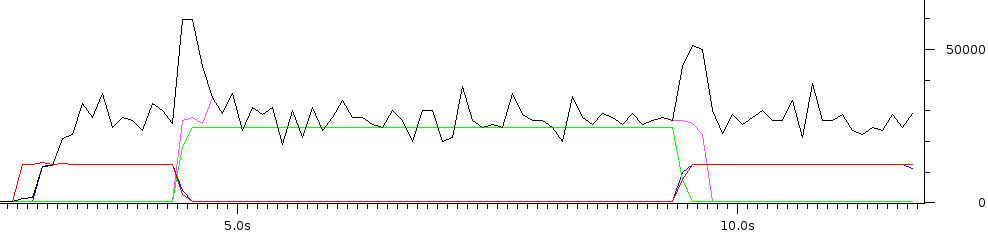
\includegraphics[width=\textwidth]{2trein3rau}
    \caption{Pakketstromen tussen de centrale en de RAU's in het RoF-model.  De horizontale as is de tijdsas, verticaal staat de doorstroom in \textit{Bytes per tick}.  E�n tick is 0,1~s waardoor de waarde 50.000 op de grafiek overeenkomt met 500.000~Bps of 4~Mbps.  De rode lijn geeft de hoeveelheid verkeer weer naar RAU0, terwijl de groene en blauwe dit doen voor RAU1 respectievelijk RAU2.  De paarse lijn geeft een indicatie van het verkeer afkomstig van RAU1, waar beide treinen zich op een bepaald moment samen bij bevinden.  De grootte van de totale stroom naar de centrale wordt weergegeven door de zwarte lijn.\label{RoF-2t3rau-centrale}}
  \end{center}
\end{figure}



\section{Evaluatie}
\npar Met deze resultaten hebben we aangetoond dat het moving cell concept een werkbare benadering kan zijn.  Het grote voordeel ten opzichte van de klassieke manier is dat de connectie nergens verloren gaat, de datastroom wordt nergens onderbroken.  Aan een dergelijke bewegingssnelheid is een connectie met traditionele WiFi-oplossingen helemaal onmogelijk, maar dit kan via het hier voorgestelde model verholpen worden.